\section{Introduction}
\label{sec:intro}

%% infographics is useful
%Infographics use a combination of graphics, text, images, and data to inform and engage.
%In animated infographics, some elements are animated to illustrate data or emphasize key points more excitingly and engagingly.
%% animated infographics are useful
Animated infographics is considered a powerful tool for storytelling. 
It has been widely used in multiple areas, such as business, publicity, science popularization and so on. 
Compared to static infographics, it can interpret data or ideas more vividly and grabs the audience's attention quickly, appreciated and shared by people for years~\cite{blazer2019animated, brehmer2016timelines}. % [5, 10] in "Communicating with Motion: A Design Space for Animated Visual Narratives in Data Videos"

% introduce existing approaches and shortcomes
%Unfortunately, the creation of animated infographics is tedious and time-consuming, especially for novice users~\cite{amini2016authoring, hullman2013deeper, shi2021communicating}. %[5 dataclip, 41, 80, in Katika]
%It can take weeks to authorize graphical animation itself that lasts around one minute \cite{howlong}.
%\qmhl{Creating animated inforgraphics from scratch involve two major steps: static inforgraphics designing and animation creating~\cite{jahanlou2020challenges, shi2021communicating}.}
%Initially, designers need to create static infographics (like te rightmost figure in \autoref{fig:ani_example}(A)) using feature-rich software such as Adobe Illustrator~\cite{AdobeAI} and  export them as Scalable Vector Graphics (SVGs) or other kinds of files so that downstream tools can be employed for animation creation.
%Then, the interactive tools (\eg Adobe After Effects~\cite{AdobeAE}) are used to add animations.
%However, they only provide low-level operations, like keyframes or interpolation, for motion authoring, which requires expertise and is time-consuming \cite{jahanlou2020challenges}.
%Some users might choose programming tools (\eg D3~\cite{bostock2011d3}) because they can precisely control property changes and organize timelines through program flow.
%In recent years, declarative languages are preferred by designers for this task as they favor conciseness over expressiveness~\cite{mcnutt2023nogrammar}. 
%Canis~\cite{ge2020canis} falls into this category, which provides a declarative language for creating animated charts.
%These techniques simplify the creation process but can only use a predefined library of simple animations usually, which limits their usage.
%Here, we introduce two examples to better illustrate the challenges of creating animated infographics with existing tools.

Crafting animated infographics is tedious and time-consuming, particularly for novice users~\cite{amini2016authoring, hullman2013deeper, shi2021communicating}. The process to produce just one minute of graphical animation can span several weeks \cite{howlong}.
The construction of animated infographics fundamentally comprises two primary stages: designing static infographics and creating animation~\cite{jahanlou2020challenges, shi2021communicating}. Initially, designers employ feature-rich software like Adobe Illustrator~\cite{AdobeAI} to craft static infographics (as exemplified by the rightmost figure in \autoref{fig:ani_example}(A)). Subsequently, these are exported as Scalable Vector Graphics (SVGs) or other file types to leverage downstream tools for animation. 
In the following stage, interactive tools such as Adobe After Effects~\cite{AdobeAE} are utilized to create animations. However, these tools only offer low-level operations like keyframes or interpolation for motion authoring, which requires a significant degree of expertise and time \cite{jahanlou2020challenges}. 
%\qmpr{ Some designers might gravitate towards programming tools like D3~\cite{bostock2011d3} for the precision they offer in controlling property changes and organizing timelines through program flow.}{What's the benefits and disadvantage of D3?}
In recent years, designers have shown a preference for declarative languages due to their succinctness, even if it sometimes comes at the cost of expressiveness \cite{mcnutt2023nogrammar}. Canis \cite{ge2020canis} falls into this category, offering a declarative language tailored for crafting animated charts. 
\qmpr{These techniques simplify the creation process but can only use a predefined library of simple animations usually, which limits their usage}{Failed to clearly introduce the limitation of Canis}.
%\qmhl{Here, we introduce two examples to better illustrate the challenges of creating animated infographics with existing tools.}


% Examples

\begin{figure*}[h]
  \centering
  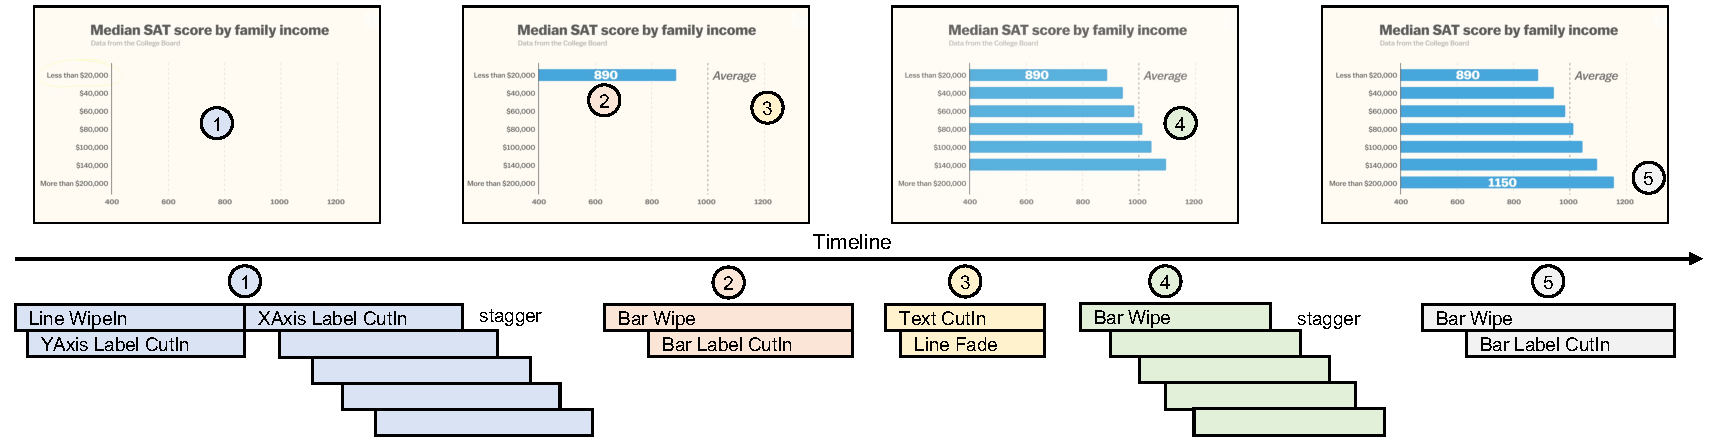
\includegraphics[width=\linewidth]{figs/ani_example_tvcg.pdf}
  \caption{(A) An animated infographic about the pretrial released defendants of the D.C. court in 2017 (retrieved from \url{https://youtu.be/5mhwDSHKEyM?t=215}). (B) An animated infographic about the relation between SAT score and family income (retrieved from \url{https://youtu.be/WjVVwMGJ9S8?t=334}). Similar animations are framed in blue. }
%  \Description{(A) An animated infographic about the pretrial released defendants of the D.C. court in 2017. (B) An animated infographic about the relation between SAT score and family income. Similar animations are framed in blue.}
  \label{fig:ani_example}
\end{figure*}

%\autoref{fig:ani_example}(A) illustrates four keyframes and the timeline of an animated.
%The creation process is as follows:
%% A1
%To implement the CutIn effect in A1, each element needs to be masked separately.
%In A1, the y coordinates of title texts should be set at the start/end keyframe to let them move out from the masks.
%% A2-3
%Then following the narration, three similar animation groups are created at the corresponding timestamp (A2-4).
%In each group, the bar enters using a Wipe effect (the mask is also required) and texts of the axis and the bar enter using CutIn.
%The relative offsets, durations and easing functions for each animation are carefully set to produce a harmonious result.

An example is shown in \autoref{fig:ani_example}(B). 
Given a static SVG shown as the rightmost figure in \autoref{fig:ani_example}(B), five animations are added (B1-5).
First, the chart framework enters at the beginning (B1) when the author explains this chart.
Similarly, animations for each element should be handled one by one, using different effects depending on the element. 
For example, the lines use the WipeIn effect, while the x-label on the left uses the CutIn effect. Increasing offsets are set for the x-axis labels to achieve the stagger effect.
Following the narration, the bar and bar label for the category "less than \$20,000" enter (B2).
A line and a label fade in to illustrate the average score (B3).
Then, bars in the middle wipe in with a stagger (B4) to show a positive correlation.
Finally, the corresponding bar and label for "More than \$200,000" are animated with similar effects (B5).

% Obstacles

Two obstacles hinder the designer's creation process. 
First, \textbf{non-intuitive and expert-driven creation approaches}. % [34, 44] in katika?
During the creation, each animation needs to: 
1) select one animation target;
2) create a start keyframe at the appropriate timestamp and set initial properties;
3) create an end keyframe at the appropriate timestamp and set final properties;
4) specify an appropriate easing function.
Designers need to deal with these cumbersome settings with an understanding of underlying concepts like keyframes, channels, \etc~\cite{krasner2013motion, sarinastiti2016skill}
This is labor-intensive but unavoidable even for experts \cite{jahanlou2020challenges}.
Second, \textbf{the repetitive creation of animations}.
We observe that animations share similarities, not only between different element groups of the same instance but also across multiple similar instances.
For example, animations framed in blue in \autoref{fig:ani_example} are similar and applied on the bars and bar labels, which can be extracted and reused.
As another example, entering animations of axes exist in many animated chart videos.
As mentioned by Thompson \etal~\cite{thompson2020understanding}, reusing animations on similar groups is useful, which simplifies and speeds up the creation process.
% conclusion
Given these situations, though these existing tools are helpful, designers of animated infographics still take a procedural approach to create them from scratch: draw the elements, select targets and create animations one by one.
% as mentioned in the work of Thompson \etal~\cite{thompson2020understanding}.
% Besides, specifying visual properties is not an intuitive way for animation creation and requires expertise~\cite{}.

% Gaia
In this work, we aim to reduce the burden of creating animated infographics greatly. 
We propose \gaia{}, a declarative \underline{\textsc{G}}rammar for \underline{\textsc{a}}nimated \underline{\textsc{i}}nfogr\underline{\textsc{a}}phics. 
\gaia{} is motivated by three goals.

\textbf{Expressivity}: \gaia{} is both expressive and intuitive for reading and writing.
In \gaia{}, animations are represented by effects applied to a group of visual elements instead of keyframes created individually for each separate element.
% insight: hierarchy of groups and animations
Groups in one infographic (as we called, instance) form a hierarchy and each group can apply effects.
Besides, grouping is also a way to organize animations~\cite{thompson2020understanding}. Animations for groups can be combined with several alignment strategies (\eg start before previous), which also form a hierarchical structure simplifying the creation and refinement of timelines. 
% Gaia
\gaia{} provides a declarative grammar following these insights, which enables designers to create animations for groups and organize them in a hierarchical timeline.
In this way, \gaia{} can support flexible and intuitive animation creation for infographics and enable users to express and refine complex animation timelines easily.
% Meanwhile, a wider variety of groups of different elements can also be animated using \gaia{}.

\textbf{Reusability}: Animations in \gaia{} can be reused.
% insight: animations share similarity
As mentioned above, reusing similar animations saves time and effort \cite{jahanlou2022katika}.
However, due to the diversity of animated objects, it is challenging even for a single simple animation, let alone a well-designed animation combo.
% Gaia
In \gaia{}, animations are declared for a class of infographics, not a concrete instance.
To this end, we conduct a target abstraction to describe graphical elements in infographics.
The animations are not directly bound to the graphical elements but instead, bound to the role of the elements in a unified representation.
For example, \gaia{} can declare a design for different types of animated elements in axes, such as domain, ticks and labels, without relying on a concrete instance.
A wide range of SVGs from the internet or other design tools can be transformed into a format that contains the roles of each animated target and other information (like data). 
Then users can reuse complex but well-designed animations from themselves or other designers.

\textbf{Extensibility}: Template library in \gaia{} can be extended.
% insight
Good design (including the coordination of effects, the design of parameters, \etcns) is difficult to express, store, and share in multiple creations.
% This is because developers are usually not professional animators.
Some existing declarative languages provide an animation library, but provided effects are preset and simple, like fade and wipe, designed for generic usage.
Meanwhile, these techniques don't provide support for extending the animation library. The only way to do this is through a code-level implementation.
% Gaia
Based on the target abstraction, \gaia{} allows expert designers to define new templates easily through a consistent declarative grammar as animation creation, then register them to the library and all users can use them just as other existing templates. 
For example, users can combine templates for bars and axes to create a new template for bar charts. 
Parameter abstraction is also introduced in \gaia{} so that a template can be more generic and customizable.

We implemented a \gaia{} compiler and released it as a TS library, which can be embedded in other tools as an animation engine with high-level specs as input.
Through a demo system with a variety of examples, we show the expressive of \gaia{}.
We conducted a user study with 8 participants with no animation design experience to illustrate the ease of use of \gaia{} and gather feedback.
All participants can acquire the core features of \gaia{} within 1h of learning, and successfully replicate the data video designed by professionals.
\gaia{} has been applied in a real-world project, and through interviews with three experts who employed it extensively, we garnered positive feedback and valuable suggestions for future improvements.

In brief, the main contributions of this work, in presentation order, include:
% \begin{enumerate}
% \item \textbf{A set of high-level grammars} that enables intuitive creation of animations (\autoref{sec:gaia_ani}). 
% Users can build complex animations via a hierarchical view and concatenating operations. 
% \item \textbf{Target abstraction} decouples animation declarations from concrete instances, enabling reusability and extendability of \gaia{}, which is the first attempt for declarative animation grammars (\autoref{sec:gaia_reuse}).
% \item \textbf{A compiler prototype} and \textbf{workflow} of \gaia{} in different points of views (\autoref{sec:workflow}).
% \item \textbf{An evaluation} on the usability of \gaia{}, including \textbf{a demo system} with multiple examples used in case studies and a user study involved both novice users and experts in animation design (\autoref{sec:eval}).
% \end{enumerate}

\squishlist 
\item \textbf{A set of high-level grammars} that enables intuitive creation of animations (\autoref{sec:gaia_ani}). 
Users can build complex animations via a hierarchical view and concatenating operations. 
\item \textbf{Target abstraction} decouples animation declarations from concrete instances, enabling reusability and extendability of \gaia{}, which is the first attempt for declarative animation grammars (\autoref{sec:gaia_reuse}).
\item \textbf{A compiler prototype}\footnote{The src code and the deployment version of both \gaia{} compiler and demo system are available in supplementary materials. An online version of the demo system is also available at \url{https://gaia-ui.azurewebsites.net}.} and \textbf{workflow} of \gaia{} in different points of views (\autoref{sec:workflow}).
\item \textbf{An evaluation} on the usability of \gaia{}, including \textbf{a demo system} with a variety of examples used in the case study, a user study involved novice users, and semi-structured interviews conducted with experts experienced in using \gaia{}.
\squishend